% tt_um_sky26c datapath -- first-order kinetic synapse driving a
% conductance-based LIF membrane.
%
% Build:  pdflatex -output-directory=. figures/datapath.tex
% Same topology as docs/datapath.svg; keep the two in sync by hand.

\documentclass[border=6pt]{standalone}
\usepackage{tikz}
\usepackage{amsmath}
\usetikzlibrary{positioning,arrows.meta,calc,fit}

\definecolor{syn}{HTML}{2A78D6}   % synapse path
\definecolor{mem}{HTML}{C2570F}   % membrane path
\definecolor{ink}{HTML}{0B0B0B}
\definecolor{muted}{HTML}{52514E}

\begin{document}
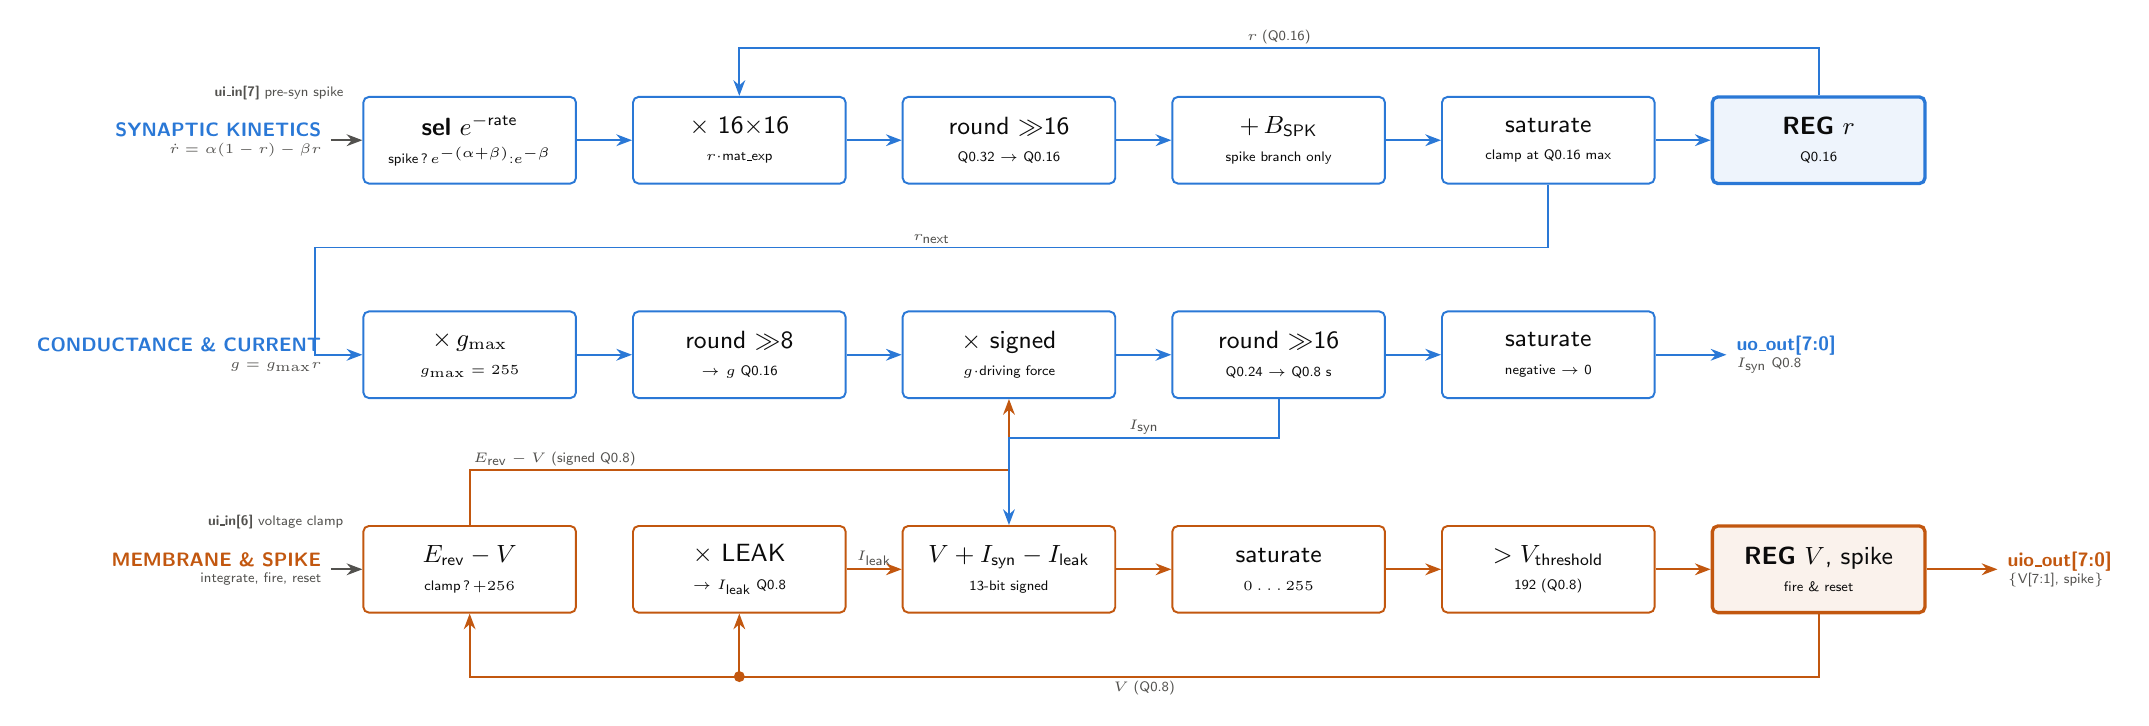
\begin{tikzpicture}[
  font=\sffamily\small,
  node distance=6mm and 7mm,
  blk/.style={draw,rounded corners=2pt,line width=0.7pt,
              minimum width=27mm,minimum height=11mm,align=center,
              inner sep=2pt,text=ink},
  syb/.style={blk,draw=syn},
  meb/.style={blk,draw=mem},
  reg/.style={blk,line width=1.2pt},
  sig/.style={-{Stealth[length=2mm]},line width=0.7pt},
  lbl/.style={font=\sffamily\tiny,text=muted,inner sep=1pt},
  lane/.style={font=\sffamily\bfseries\scriptsize},
]

% ---------------------------------------------------------------- kinetics
\node[syb]                       (a1) {\textbf{sel} $e^{-\text{rate}}$\\[-1pt]
                                       {\tiny spike\,?\,$e^{-(\alpha+\beta)}$:$e^{-\beta}$}};
\node[syb, right=of a1]          (a2) {$\times$ 16$\times$16\\[-1pt]{\tiny $r\cdot$mat\_exp}};
\node[syb, right=of a2]          (a3) {round $\gg$16\\[-1pt]{\tiny Q0.32 $\to$ Q0.16}};
\node[syb, right=of a3]          (a4) {$+\,B_{\text{SPK}}$\\[-1pt]{\tiny spike branch only}};
\node[syb, right=of a4]          (a5) {saturate\\[-1pt]{\tiny clamp at Q0.16 max}};
\node[syb, reg, draw=syn, right=of a5, fill=syn!8] (a6) {\textbf{REG} $r$\\[-1pt]{\tiny Q0.16}};

\foreach \i/\j in {a1/a2,a2/a3,a3/a4,a4/a5,a5/a6} \draw[sig,syn] (\i) -- (\j);

% r feedback, above the lane
\draw[sig,syn] (a6.north) -- ++(0,6mm) -| node[lbl,pos=0.25,above] {$r$ (Q0.16)} (a2.north);

\node[lane,text=syn,left=4mm of a1,align=right,anchor=east]
  {SYNAPTIC KINETICS\\[-2pt]{\tiny\mdseries\color{muted}$\dot r=\alpha(1-r)-\beta r$}};
\draw[sig,muted] ($(a1.west)+(-4mm,0)$) -- (a1.west);
\node[lbl,above=6mm of a1.west,anchor=east,xshift=-2mm]
  {\textbf{ui\_in[7]} pre-syn spike};

% ----------------------------------------------------- conductance, current
\node[syb, below=16mm of a1]     (b1) {$\times\,g_{\max}$\\[-1pt]{\tiny $g_{\max}=255$}};
\node[syb, right=of b1]          (b2) {round $\gg$8\\[-1pt]{\tiny $\to g$ Q0.16}};
\node[syb, right=of b2]          (b3) {$\times$ signed\\[-1pt]{\tiny $g\cdot$driving force}};
\node[syb, right=of b3]          (b4) {round $\gg$16\\[-1pt]{\tiny Q0.24 $\to$ Q0.8 s}};
\node[syb, right=of b4]          (b5) {saturate\\[-1pt]{\tiny negative $\to$ 0}};

\foreach \i/\j in {b1/b2,b2/b3,b3/b4,b4/b5} \draw[sig,syn] (\i) -- (\j);

% r_next tapped down into the conductance lane
\draw[sig,syn] (a5.south) |- ++(0,-8mm) -| ($(b1.west)+(-6mm,0)$)
  node[lbl,pos=0.25,above] {$r_{\text{next}}$} -- (b1.west);

\draw[sig,syn] (b5.east) -- ++(9mm,0)
  node[right,align=left,font=\sffamily\scriptsize]
  {\textbf{uo\_out[7:0]}\\[-2pt]{\tiny\color{muted}$I_{\text{syn}}$ Q0.8}};

\node[lane,text=syn,left=4mm of b1,align=right,anchor=east]
  {CONDUCTANCE \& CURRENT\\[-2pt]{\tiny\mdseries\color{muted}$g=g_{\max}r$}};

% -------------------------------------------------------- membrane, spike
\node[meb, below=16mm of b1]     (c1) {$E_{\text{rev}}-V$\\[-1pt]{\tiny clamp\,?\,$+256$}};
\node[meb, right=of c1]          (c2) {$\times$ LEAK\\[-1pt]{\tiny $\to I_{\text{leak}}$ Q0.8}};
\node[meb, right=of c2]          (c3) {$V+I_{\text{syn}}-I_{\text{leak}}$\\[-1pt]{\tiny 13-bit signed}};
\node[meb, right=of c3]          (c4) {saturate\\[-1pt]{\tiny $0\ldots255$}};
\node[meb, right=of c4]          (c5) {$>V_{\text{threshold}}$\\[-1pt]{\tiny 192 (Q0.8)}};
\node[meb, reg, draw=mem, right=of c5, fill=mem!8] (c6) {\textbf{REG} $V$, spike\\[-1pt]{\tiny fire \& reset}};

\draw[sig,mem] (c2) -- node[lbl,above] {$I_{\text{leak}}$} (c3);
\foreach \i/\j in {c3/c4,c4/c5,c5/c6} \draw[sig,mem] (\i) -- (\j);

% driving force up into the current lane
\draw[sig,mem] (c1.north) -- ++(0,7mm)
  node[lbl,above right] {$E_{\text{rev}}-V$ (signed Q0.8)} -| (b3.south);
% I_syn down into the membrane sum
\draw[sig,syn] (b4.south) -- ++(0,-5mm) -| node[lbl,pos=0.25,above] {$I_{\text{syn}}$} (c3.north);

% V feedback, below the lane
\draw[sig,mem] (c6.south) -- ++(0,-8mm) -| node[lbl,pos=0.25,below] {$V$ (Q0.8)} (c1.south);
\draw[sig,mem] ($(c2.south)+(0,-8mm)$) -- (c2.south);
\fill[mem] ($(c2.south)+(0,-8mm)$) circle (0.7mm);

\draw[sig,mem] (c6.east) -- ++(9mm,0)
  node[right,align=left,font=\sffamily\scriptsize]
  {\textbf{uio\_out[7:0]}\\[-2pt]{\tiny\color{muted}\{V[7:1], spike\}}};

\node[lane,text=mem,left=4mm of c1,align=right,anchor=east]
  {MEMBRANE \& SPIKE\\[-2pt]{\tiny\mdseries\color{muted}integrate, fire, reset}};
\draw[sig,muted] ($(c1.west)+(-4mm,0)$) -- (c1.west);
\node[lbl,above=6mm of c1.west,anchor=east,xshift=-2mm]
  {\textbf{ui\_in[6]} voltage clamp};

\end{tikzpicture}
\end{document}
